%----------------------------------------------------------------------------------------
%	PACKAGES AND OTHER DOCUMENT CONFIGURATIONS
%----------------------------------------------------------------------------------------

\documentclass[
	11pt, % Set the default font size, options include: 8pt, 9pt, 10pt, 11pt, 12pt, 14pt, 17pt, 20pt
	%t, % Uncomment to vertically align all slide content to the top of the slide, rather than the default centered
	aspectratio=169, % Uncomment to set the aspect ratio to a 16:9 ratio which matches the aspect ratio of 1080p and 4K screens and projectors
	envcountsect,
	xcolor=dvipsnames
]{beamer}

\usepackage{PresentationTemplate}

\graphicspath{{Images/}{./}} % Specifies where to look for included images (trailing slash required)
%----------------------------------------------------------------------------------------
%	PRESENTATION INFORMATION
%----------------------------------------------------------------------------------------

\title[CVE101 - Civil Engineering Orientation]{Lecture 2} % The short title in the optional parameter appears at the bottom of every slide, the full title in the main parameter is only on the title page

\subtitle{KEYS TO SUCCESS IN CIVIL ENGINEERING STUDY} % Presentation subtitle, remove this command if a subtitle isn't required

\author[Nikol O. Telen]{Nikol O. Telen} % Presenter name(s), the optional parameter can contain a shortened version to appear on the bottom of every slide, while the main parameter will appear on the title slide

\institute[MSU-GenSan, Civil Engineering Department
]{{\scriptsize Mindanao State University - General Santos}\\\textbf{CIVIL ENGINEERING DEPARTMENT}} % Your institution, the optional parameter can be used for the institution shorthand and will appear on the bottom of every slide after author names, while the required parameter is used on the title slide and can include your email address or additional information on separate lines

\date{\today} % Presentation date or conference/meeting name, the optional parameter can contain a shortened version to appear on the bottom of every slide, while the required parameter value is output to the title slide

\titlegraphic{
	
\includegraphics[width=1cm]{MSU.jpg}
	\hspace{0.2cm}
	
\includegraphics[width=1cm]{CEdept.png}
} 

\institute[MSU-GenSan, Civil Engineering Department]{{\scriptsize Mindanao State University - General Santos}\\\textbf{CIVIL ENGINEERING DEPARTMENT}}
\date{\today} 
\subject{CVE101 - Civil Engineering Orientation}

%----------------------------------------------------------------------------------------

\begin{document}

%----------------------------------------------------------------------------------------
%	TITLE SLIDE
%----------------------------------------------------------------------------------------

\begin{frame}
	\titlepage % Output the title slide, automatically created using the text entered in the PRESENTATION INFORMATION block above
\end{frame}

%----------------------------------------------------------------------------------------
%	TABLE OF CONTENTS SLIDE
%----------------------------------------------------------------------------------------

% The table of contents outputs the sections and subsections that appear in your presentation, specified with the standard \section and \subsection commands. You may either display all sections and subsections on one slide with \tableofcontents, or display each section at a time on subsequent slides with \tableofcontents[pausesections]. The latter is useful if you want to step through each section and mention what you will discuss.

\begin{frame}
	\frametitle{Lecture Overview} % Slide title, remove this command for no title
	
	\tableofcontents % Output the table of contents (all sections on one slide)
	%\tableofcontents[pausesections] % Output the table of contents (break sections up across separate slides)
\end{frame}

%----------------------------------------------------------------------------------------
%	PRESENTATION BODY SLIDES
%----------------------------------------------------------------------------------------

\section{Potential for Success}
\SectionPage
	\begin{frame}[plain]
		\begin{figure}
			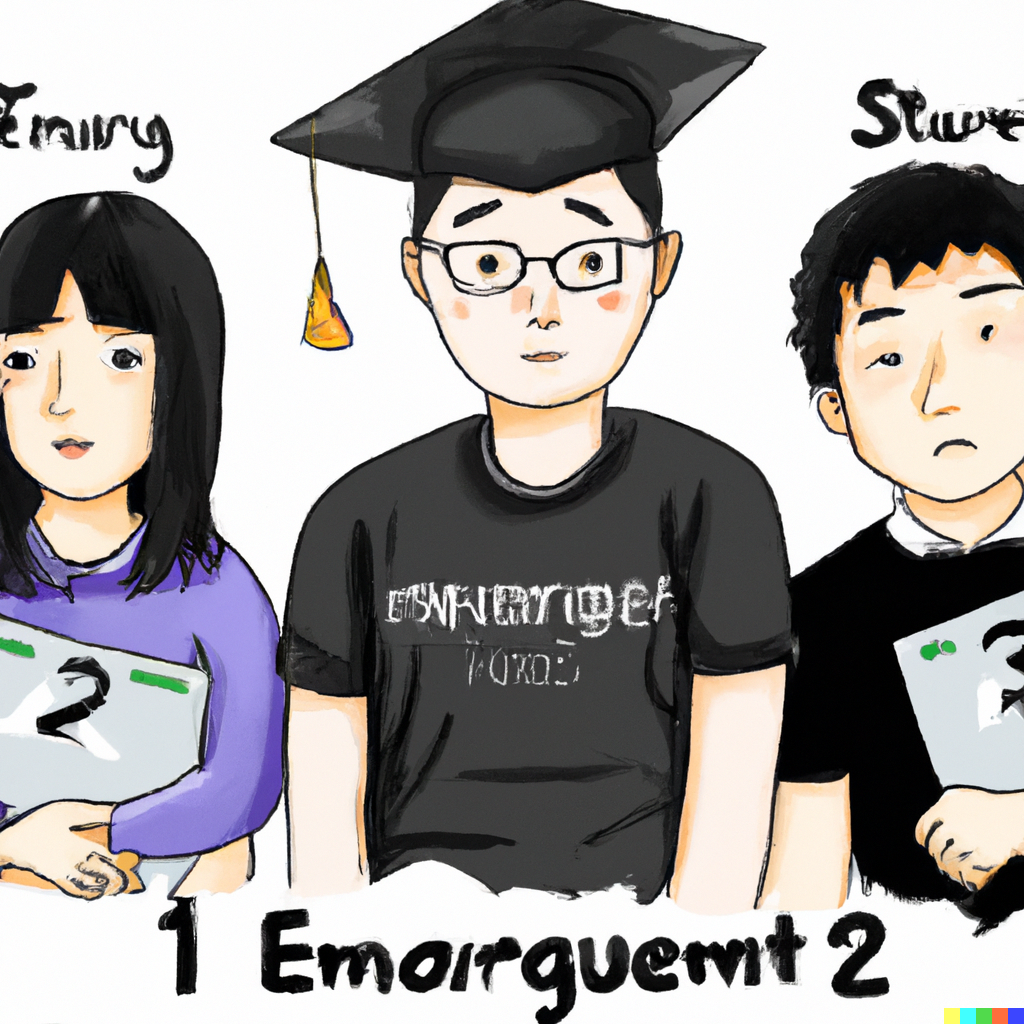
\includegraphics[width=0.55\linewidth]{graduates.png}
			%\caption{Creodocs logo.}
		\end{figure}
	\end{frame}

	\begin{frame}
		\begin{quote}
			"Each and every one of you has the potential to successfully graduate and 
			earn your BS in Civil Engineering degree"\\
			--- Someone, somewhere, sometime\ldots
		\end{quote}
	\end{frame}

	\begin{frame}
		\begin{columns}[c] % The "c" option specifies centered vertical alignment while the "t" option is used for top vertical alignment
			\begin{column}{0.45\textwidth} % Left column width
				\begin{quote}
					Poorly prepared students have succeeded
				\end{quote}
			\end{column}

			\begin{column}{0.5\textwidth} % Right column width
				\begin{figure}
					
\includegraphics[width=1\linewidth]{billgates.jpg}
				\end{figure}
			\end{column}
		\end{columns}
	\end{frame}

	\begin{frame}
		\begin{columns}[c] % The "c" option specifies centered vertical alignment while the "t" option is used for top vertical alignment
			\begin{column}{0.45\textwidth} % Left column width
				\begin{figure}
					
\includegraphics[width=1\linewidth]{badluckbrian.jpg}
				\end{figure}
			\end{column}

			\begin{column}{0.5\textwidth} % Right column width
				\begin{quote}
					Highly qualified students have failed
				\end{quote}
			\end{column}
		\end{columns}
	\end{frame}

	\begin{frame}[plain] % The optional argument 'plain' hides the headline and footline
		\begin{center}
			{\Huge What happened?}
			
			\bigskip\bigskip % Vertical whitespace
			
			{\LARGE How can a student succeed or fail.??? }
		\end{center}
	\end{frame}

	\begin{frame}{Potential for Success}
		A reason for their failure is \alert{Overconfidence}.\\
		\bigskip 
		Those who succeeded definitely found a way to become an "expert" on success.\\
		\bigskip
		And it's something that anyone can do.
	\end{frame}

	\begin{frame}[plain] % The optional argument 'plain' hides the headline and footline
		\begin{center}
			{\Huge What is success?}
			
			\bigskip\bigskip % Vertical whitespace
			
			{\LARGE ??? }
		\end{center}
	\end{frame}

	\begin{frame}
	\frametitle{What is success?}
		\visible<1->{
			\begin{quote}\ldots generally refers to the achievement of a desired outcome or the 
			realization of a particular goal\\
			--- ChatGPT 3.5, August 2023
			\end{quote}
		}
	\end{frame}

	\begin{frame}
	\frametitle{What is success?}
		\visible<1->{
			\begin{quote}
				there can never be success without desire, plan, or attempt
			\end{quote}
		}
	\end{frame}

	\begin{frame}
		According to Vincent Tinto, the top two reasons why students do not succeed college are:
			\begin{enumerate}
				\item<2-> Lack of intention - \visible<3->{students do not have a clear educational and/or career goal}
				\item<4-> Lack of commitment - \visible<5->{students do not have motivation and 
				drive to work toward attaining their goal}
			\end{enumerate}
	\end{frame}

	\begin{frame}
		Identifying a clear goal, and committing to it are the two most important steps in attaining success.
	\end{frame}
	
\section{Foundations of Success}
\SectionPage
	\begin{frame}
		\frametitle{Goal Setting}
		Have specific ideas what you want to accomplish in short and long term. With this 
		you will be able to:
		\begin{enumerate}
			\item<2-> Have a direction in life
			\item<3-> Have something to measure your progress with
		\end{enumerate}	
	\end{frame}

	\begin{frame}[plain] % The optional argument 'plain' hides the headline and footline
		\begin{center}
			{\Huge So what is your Goal?}
			
			\bigskip\bigskip % Vertical whitespace
			
			{\LARGE Short Term? Medium Term? Long Term?}
		\end{center}
	\end{frame}

	\begin{frame}
	\frametitle{Making a Commitment}
			Regardless of your reasons for selecting Civil Engineering, it is important
			to develop a strong motivation to succeed.

			\bigskip

			Civil Engineering is a very demanding field of study. Even students with excellent
			preparation and strong ability will not succeed without a high level of commitment
	\end{frame}

	\begin{frame}
		\begin{columns}[c] % The "c" option specifies centered vertical alignment while the "t" option is used for top vertical alignment
			\begin{column}{0.45\textwidth} % Left column width
				\begin{figure}
					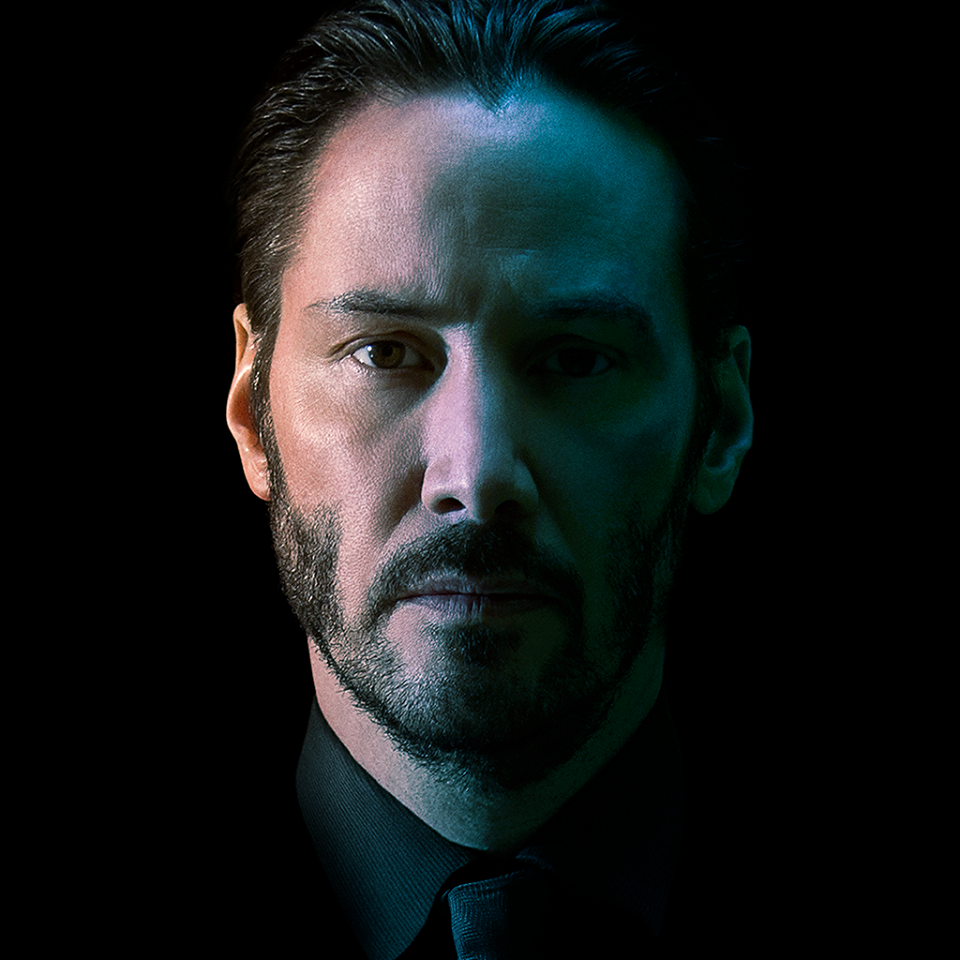
\includegraphics[width=1\linewidth]{johnwick.png}
				\end{figure}
			\end{column}
			
			\begin{column}{0.5\textwidth} % Right column width
				He Is a Man of 
				\begin{itemize}
					\item<2-> Focus
					\item<3-> Commitment
					\item<4-> and Sheer F****** Will
				\end{itemize}
			\end{column}
		\end{columns}
	\end{frame}

	\begin{frame}
	\frametitle{Strengthening your Commitment}
		The following strategies can help in strengthening your commitment:
		\begin{itemize}
			\item Clarify your goals
			\item Learn as much as you can about Civil Engineering
			\item Prepare a road map
			\item Don't let adversity stop you 
		\end{itemize}
	\end{frame}

	\begin{frame}
		\frametitle{Clarifying Goals}
		\framesubtitle{Strengthening your Commitment}
			Clarifying goals helps you understand their value to you.\\
			\bigskip
			By better understanding their value, the more you become committed to your goal 
	\end{frame}

	\begin{frame}
		\frametitle{Learning more about Civil Engineering}
		\framesubtitle{Strengthening your Commitment}
			Increased knowledge brings increased motivation.\\
			\bigskip
			We tend to like things we know a lot about.
	\end{frame}

	\begin{frame}
		\frametitle{Know where to go}
		\framesubtitle{Strengthening your Commitment}
			Develop a "road map" that will lead you to graduate in Civil Engineering.\\
			\bigskip
			Knowing the subjects you need to take, and how they relate to the subjects you're
			currently taking boosts your commitment to succeed on it.
	\end{frame}

	\begin{frame}
		\frametitle{Don't let adversity stop you }
		\framesubtitle{Strengthening your Commitment}
			Strengthened commitment develops determination.\\
			\bigskip
			Determination means having an unwavering commitment to your goal: 
			the goal of graduating in Civil Engineering
	\end{frame}

\section{Keys to Success}
\SectionPage
	\begin{frame}{Keys to Success}
		Setting a goal and making it important to you are only the first steps.\\
		\bigskip
		The real challenge remains - achieving the goal.
	\end{frame}

	\begin{frame}{Keys to Success}
		Once your goal is identified and you have done everything you can to develop
		a strong commitment to that goal, achieving it requires that you adjust both 
		your attitudes and your behaviors\\
	\end{frame}

	\begin{frame}{Keys to Success}
		\begin{itemize}
			\item<1-> Attitude - "Think positively"
			\item<2-> Approach - "Work Smart"
			\item<3-> Effort - "Work Hard"
		\end{itemize}
	\end{frame}

	\begin{frame}{Attitude - Think Positively}
		\framesubtitle{Keys to Success}
			Positive attitudes produce positive results. Negative attitudes produce negative results.
	\end{frame}

	\begin{frame}{Attitude - Think Positively}
		\framesubtitle{Keys to Success}
		Among those negative attitudes that could produce negative 
		results in engineering study are:
		\begin{columns}[c] % The "c" option specifies centered vertical alignment while the "t" option is used for top vertical alignment
			\begin{column}{0.45\textwidth} % Left column width
				\begin{itemize}
					\item<2-> Overconfidence
					\item<3-> Low self-confidence
					\item<4-> Lack of self-worth
					\item<5-> External “locus-of-control”
					\item<6-> Unwillingness to seek help
				\end{itemize}
			\end{column}
			
			\begin{column}{0.5\textwidth} % Right column width
				\begin{itemize}
					\item<7-> Resistance to change your behaviors and attitudes
					\item<8-> Tendency to procrastinate
					\item<9-> Avoidance of areas of weakness
					\item<10-> Reluctance to study with other students
					\item<11-> Negative view toward authority figures
					\item<12-> Weak commitment to the goal of graduating in engineering
				\end{itemize}
			\end{column}
		\end{columns}
	\end{frame}

	\begin{frame}{Approach - Work Smart}
		\framesubtitle{Keys to Success}
		Approach refers to how you go about your engineering studies.\\
		\bigskip
		It means that you work not only hard, but smart.\\
	\end{frame}

	\begin{frame}{Approach - Work Smart}
		\framesubtitle{Keys to Success}
		Your approach to the study of engineering can be likened to a game.\\
		\bigskip
		To become a pro gamer (i.e., master student), you must not only play the game (i.e., be a student);\\
		\bigskip
		you must also devote time and energy to learning how to play it (i.e., learn to excel as a student).
	\end{frame}

	\begin{frame}{Effort - Work Hard}
		\framesubtitle{Keys to Success}
			People succeed not because of their ability. People succeed because of their effort.\\
			\bigskip
			Effort involves committing time and energy.\\
			\bigskip
			Accomplishing an academic task, like completing a homework assignment, 
			will require you to devote adequate time and to focus your mental energy. 
			These are things that you can choose to do or choose not do.
	\end{frame}

\section{Summary}
\SectionPage
	\begin{frame}{Summary}
		The steps to the "success process" is:
		\begin{enumerate}
			\item \textbf{Setting goals} - Do I want to be a civil engineer?
			\item \textbf{Strengthening commitment to goals} - How important is it to me to become an engineer?
			\item \textbf{Changing negative attitudes} - What attitudes will interfere with my goal of becoming an engineer?
			\item \textbf{Changing non-productive behaviors} - What do I need to do differently to achieve my goal of becoming an engineer?
		\end{enumerate}
	\end{frame}

%------------------------------------------------

%\begin{frame} % Use [allowframebreaks] to allow automatic splitting across slides if the content is too long
%	\frametitle{References}
%	
%	\begin{thebibliography}{99} % Beamer does not support BibTeX so references must be inserted manually as below, you may need to use multiple columns and/or reduce the font size further if you have many references
%		\footnotesize % Reduce the font size in the bibliography
%		
%		\bibitem[Smith, 2022]{p1}
%			John Smith (2022)
%			\newblock Publication title
%			\newblock \emph{Journal Name} 12(3), 45 -- 678.
%			
%		\bibitem[Kennedy, 2023]{p2}
%			Annabelle Kennedy (2023)
%			\newblock Publication title
%			\newblock \emph{Journal Name} 12(3), 45 -- 678.
%	\end{thebibliography}
%\end{frame}


%----------------------------------------------------------------------------------------
%	CLOSING SLIDE
%----------------------------------------------------------------------------------------

\begin{frame}[plain] % The optional argument 'plain' hides the headline and footline
	\begin{center}
		{\Huge The End}
		
		\bigskip\bigskip % Vertical whitespace
		
		{\LARGE Questions? Comments?}
	\end{center}
\end{frame}

%----------------------------------------------------------------------------------------
\end{document} 